\section{Extending the \METHOD~Structured Language}
\label{section:extendability}



\begin{figure*}[t]
    \centering
    \includegraphics[height=8cm]{example-image-duck}
    \caption{Main Qualitative results. Showing Comparisons with SceneCAD and Roomformer for layout prediction, and with Mask3D or others for object detection. @ARMEN will fill this up.}
    \label{fig:enter-label}
\end{figure*}

In this section, we showcase how our language can be made more expressive to represent non-planar entities, composition of entities, and object states. Additionally, we show how our language can be easily extended to handle coarse 3D object reconstruction.

It is worth noting that for each of the following proof-of-concept experiments, \textbf{only} a change to the \METHOD~language was required. All other experimental factors (e.g. architecture, training config) were constant, demonstrating a significantly lower barrier to entry than previous methods which often require additional engineering for each novel task.

\subsection{Extending \METHOD~with Curved Entities}

Previous works often employ heuristics
limiting them to specific scene entities.
For example,
methods based on planes such as \cite{furukawa2009reconstructing,liu2019planercnn}
typically utilize robust estimation procedures custom tailored to planar primitive fitting.
Extending such methods to more complex entities is non-trivial and requires significant effort.
In contrast,
our structured language-based approach makes it straightforward to extend to curved walls,
as for example extruded Bezier curves~\cite{beziercurves}.
To do this,
we define a new entity called \texttt{make\_curved\_wall}. 

The curved wall command is a simple Bezier parametrization
consisting of 4 additional parameters:
the $x,y$ values of the 2 control points
that define the wall curvature.
Explicitly, our planar wall command changes to: 
\begin{lstlisting}[language=StructuredLanguage]
make_curved_wall: a_x, a_y, a_z, b_x, b_y, b_z, c1_x, c2_y, c2_x, c2_y, height, thickness
\end{lstlisting}
where $c_{1_x}, c_{1_y}, c_{2_x}, c_{2_y}$ are the Bezier control points. 


We generate a synthetic curved walls dataset to train \METHOD.
Example Bezier walls with a qualitative evaluation are in Figure~\ref{fig:extensions} (left).
The predictions are nearly indistinguishable compared to ground truth,
indicating that our method can learn to predict such complex primitives.

\subsection{Extending \METHOD~to Compositions of Wall Primitives}

To further explore the limits of our \METHOD,
we turn our attention into the problem of representing complexly shaped walls
as compositions of cuboids.
We define a new parametrization for this class of walls as follows:
\begin{lstlisting}[language=StructuredLanguage]
make_wall: a_x, a_y, ...
make_wall_prim: pos_x, pos_y, pos_z, size_x, size_y, size_z
\end{lstlisting}
where the \lstinline[style=cmdstyle]!make_wall_prim! command describes a cuboid
to be composed with its parent wall entity.
We added such cuboid compositions to a base wall
in Figure~\ref{fig:extensions} (left).
In this proof-of-concept,
the results clearly demonstrate the ability of the network
to infer compositions of cuboids on base walls
only from a noisy surface point cloud.


  
\subsection{Extending \METHOD~to Object States}

To illustrate the flexibility of our method, we showcase how trivially we can add entity state estimation to our pipeline. Yet another simple extension to our \METHOD~language allows us to represent door states, w.r.t their opening configuration. For this, we simply change the original door representation to include a list of parameters that define door state as follows:

\begin{figure*}[t]
    \centering
    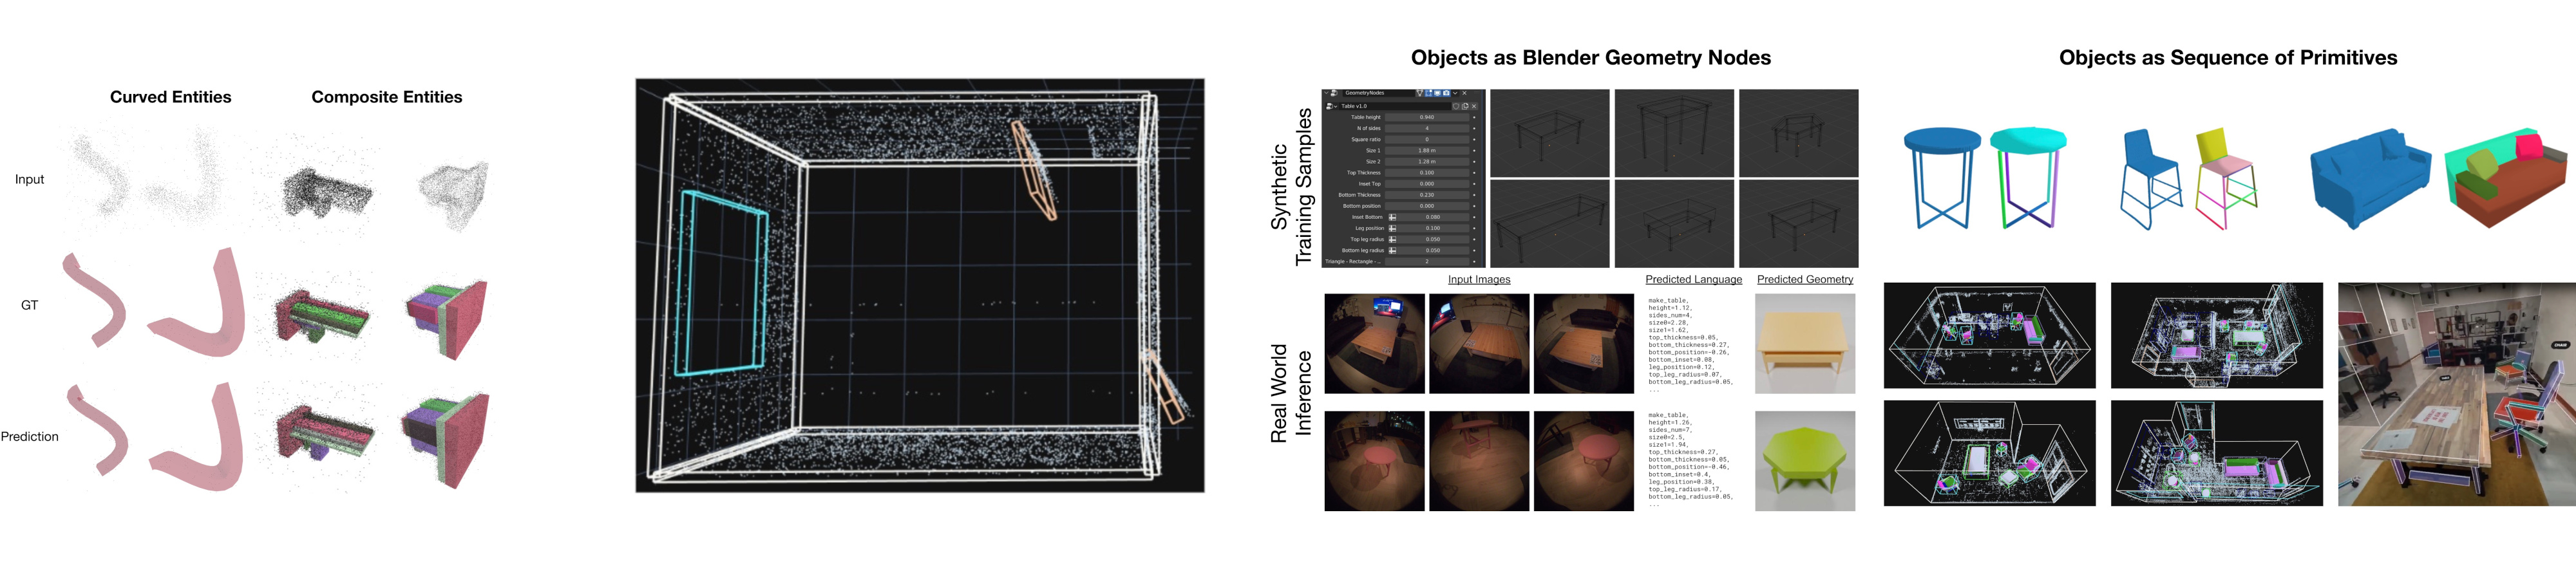
\includegraphics[width=\textwidth]{figs/new_final.jpg}
    \caption{Extending the \METHOD~ language to multiple novel tasks. a) Non-planar wall reconstruction b) Entity state estimate (door opening angle) c) Object Reconstruction using Blender Geometry Nodes d) Object Reconstruction using geometric primitive decomposition. We can observe that our method is able to handle multiple novel tasks with success (without any changes in the network architecture and training process), which illustrates its suitability as a generic scene reconstruction methodology. [WIP WILL beautify the figure later today]}
    \label{fig:extensions}
\end{figure*}


\begin{lstlisting}[language=StructuredLanguage]
make_door: id, wall_id, pos_x, pos_y, pos_z, width, height, open_degree, hinge_side, open_direction
\end{lstlisting}
\texttt{hinge\_side} represents which side of the door the hinge is on, \texttt{open\_direction} determines whether the door opens into the room or outside of the room, and \texttt{open\_degree} is the angle of the opening.
In Figure~\ref{fig:extensions} (second),
we qualitatively demonstrate object state estimation.
We annotated our doors
with a new command parameterization
extended by door hinge position, wall opening side and opening angle.
As with our other extensions,
our model is able to handle this situation without issue.
This small GT language extension demonstrates effective state estimation
while the input and network architecture remain unchanged.

\subsection{Extending \METHOD~to Reconstruct Objects}

Up to now, we have been focusing on showcasing the efficacy of \METHOD~for representing simple layout elements and objects as bounding boxes. In this section, we illustrate that just a few minor extra definitions allow our method to additionally reconstruct objects at a higher detail level compared to bounding boxes. We explore two different ways to do that: 1) blender geometry nodes 2) object primitive decomposition.

\subsubsection{Blender Parametric Object Models}

Parametric modelling offers detailed high-quality geometry representations along with interpretability and editability by design~\cite{jones2020shapeassembly,jones2021shapemod,jones2022plad,pearl2022geocode}. 
The Blender community offers readily accessible Geometry Nodes of diverse object categories as a procedural language.
We investigate the use of a particular Geometry Node for tables~\cite{mrBash2023Tables},
shown in Figure~\ref{fig:extensions} (right center).
Not only can we directly incorporate this parametric model
into our \METHOD~language,
but we can also use it to generate data
by randomly sampling its parameters
similar to~\cite{pearl2022geocode}. 

We design a simple proof-of-concept experiment where we render synthetic RGB images of random tables, composite them on a random image background, and learn to predict the ground truth Blender procedural language.
In Figure~\ref{fig:extensions} (right center), we demonstrate two real-world inferences of tables using this language, showing our method is capable of predicting reasonable parameters to reconstruct these tables. Interestingly, in the second example the model predicts a high \texttt{sides\_num} to approximate the circular tabletop, which was not on the training set.

\subsubsection{Objects as Geometric Primitives Sequences}

While the above approach of parametric object modelling is effective, it requires a separate language definition for each object category. To minimize such effort, an alternative approach would be to design a language that can describe many object categories simultaneously while still maintaining a reasonable level of semantics.


We turn to a language based on volumetric primitives, motivated by works such as~\cite{tulsiani2017learning,yang2021unsupervised}. Using simple primitives such as cuboids and extruded cylinders, we can coarsely represent arbitrary object categories while maintaining object semantics (e.g. tabletops can be represented by a single cuboid). To do this, we additionally define the following command:

\begin{lstlisting}[language=StructuredLanguage]
make_prim: bbox_id, prim_num, class, center_x, center_y, center_z, angle_x, angle_y, angle_z, scale_x, scale_y, scale_z
\end{lstlisting}

To obtain ground truth \lstinline[style=cmdstyle]!make_prim! commands that align with the objects in \DatasetName, we first run an extension of Yang. et al~\cite{yang2021unsupervised} to obtain cuboid and extruded cylinder primitives of a database of 3D CAD models (ABO~\cite{collins2022abo}, which was used to populate \DatasetName). See Figure~\ref{fig:extensions} (right center) for example decompositions. For this proof-of-concept experiment, we use three categories: \textit{table}, \textit{chair}, and \textit{sofa}. We then convert these decomposed primitives into \lstinline[style=cmdstyle]!make_prim! commands that are aligned with the objects in the dataset, which results in training pairs. Again, note that the point clouds and architecture remain the same, and only the ground truth language is augmented with new commands.

In Figure~\ref{fig:extensions} (right),
we show inferences in a few real-world environments
despite only having trained on our simulated dataset.
The results show that our method is capable of coarsely reconstructing objects of multiple categories.
Importantly, recall that the joint inference of both layout elements and coarse object reconstruction are done with a single general purpose architecture.
